\begin{frame}[t]{The LHCb experiment (1)}
\small
\centering
\begin{columns}[t]
\column{.5\textwidth}
Forward spectrometer with planar detectors:
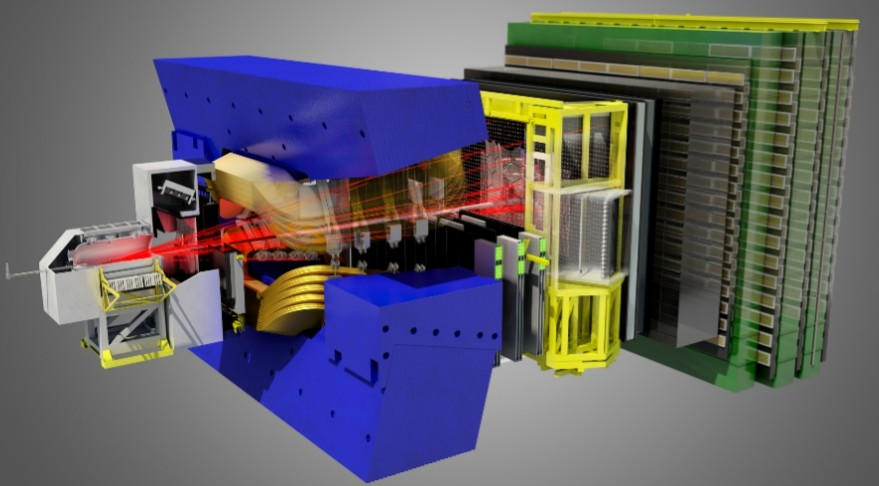
\includegraphics[width=.9\textwidth]{lhcb/lhcb-general}

\begin{itemize}
\item \textcolor{red}{LHCb uniqueness:}
\begin{itemize}
\footnotesize
\item Tracking, RICH and calorimeters cover
the full detector acceptance ($2.0< \eta <5.0$);
tracking coverage also in the backward
region ($-4.0 < \eta <-1.5$)
\item Covers just ~4\% of the solid angle but captures
~25\% of heavy quark pairs produced at the \lhc.
\item Ability to study low-pT processes at large $\eta$
\end{itemize}
\end{itemize}

\column{.5\textwidth}
Heavy quark pair production at the \lhc:
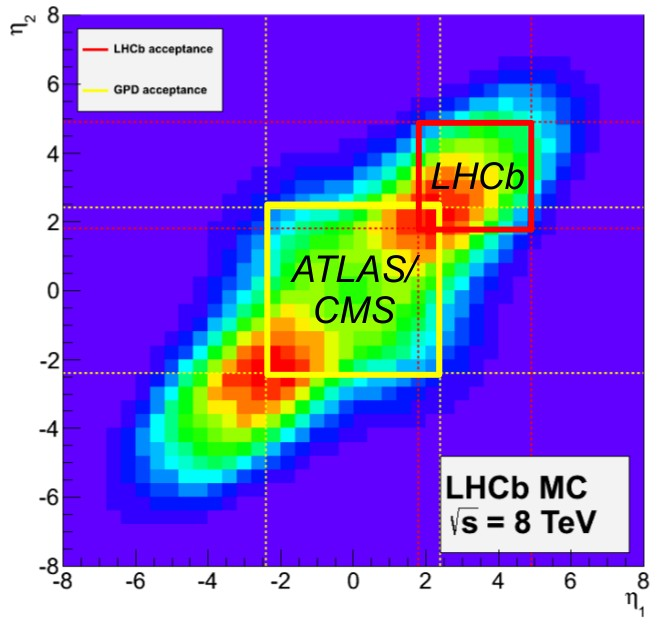
\includegraphics[width=.9\textwidth]{lhcb/bb-range}

Fraction of $b\bar{b}$ pairs in the acceptance:
\resizebox{.9\textwidth}{!}{
\begin{tabular}{rrr}\toprule
\sqs & \atlas/\cms & \lhcb\\
\midrule
7\tev & 44\% & 25\%\\
14\tev & 41\% & 24\%\\
\bottomrule
\end{tabular}
}
\end{columns}

\end{frame}